\chapter{Conclusions}

The \alphat search for SUSY has been presented using a 12.9 \ifb 
dataset of 13 \TeV~p-p collisions collected by the CMS experiment. 
The search uses a hadronic final state containing jets and 
significant~\met to achieve sensitivity to a wide range of SUSY
models. Dedicated variables, including \alphat and \bdphi, are used 
to mitigate backgrounds and remaining contributions
are robustly estimated using simulation and control regions in data.
The results of the \alphat search following the strategy
described in this thesis have been published using 
a 2.3 \ifb dataset collected in 2015~\cite{alphat2015} while the results 
of a search using the full 36 \ifb dataset collected by CMS in 2016 
are being prepared for publication.

Earlier incarnations of the \alphat~analysis have been carried out
on datasets of 8 \TeV~p-p collisions. The analysis has been
fully updated and extended for the results presented in this thesis. 
In particular, the addition of the \mht dimension has robustly improved the sensitivity of the search. 
No evidence for BSM physics is observed and the results are 
therefore interpreted using simplified SUSY models. As shown in Chapter~\ref{cha:statisticalResults},
the regions of parameter space excluded for both gluino mediated 
and direct bottom and top squark production have been 
significantly extended.

The \alphat search is sensitive to models not considered in the
interpretations presented in this thesis. Such models include 
complete models of SUSY and generic models of dark matter. 
A procedure for facilitating the re-interpretation of the results of the search to evaluate the 
impact on such models has been presented. This procedure 
may be applied to a wide range of searches for BSM physics~\cite{simp-lik}.

The L1 trigger jet and energy sum algorithms have been
developed to take advantage of the upgraded L1 trigger hardware.
These provide improved performance in jet identification, 
reconstruction and pileup mitigation. The upgraded algorithms have
been in use for the full 2016 dataset and have been exploited
by the \alphat analysis in designing inclusive signal region selections.

No evidence has been found for BSM physics in the \alphat analysis 
or any search at CMS. The improvements to the analysis and substantial
increase in centre of mass energy has provided significant gains in
the excluded parameter space for hadronic SUSY models. 

The bounds on masses of gluinos and squarks at 1 - 2 \TeV~ imply fine
tuning at the percentage level~\cite{hmus} for a generic MSSM scenario. 
While this does not provide strong evidence for the non-existence of SUSY,
the motivation for gluinos and squarks in a mass range that may be explored 
by the LHC is significantly weakened.  

There are many alternatives to the `vanilla' MSSM which remain well-motivated 
and give rise to detectable signatures at the LHC. These include RPV models,
which do not include a DM candidate but evade constraints from searches which require \met~\cite{rpv}, 
`hidden valley' models~\cite{hValley}, which typically lead to signatures with little \met and multiple
soft jets, and `split SUSY' which leads to long-lived particle signatures~\cite{sSusy}.

Finally, it is important to emphasise that naturalness is not the only motivation
for observable SUSY. Experimental observations and constraints, such as the Higgs discovery~\cite{cmsHiggs,atlasHiggs},
and the anomolous magnetic moment of the muon~\ref{gm2}, constrain the parameter
space of full SUSY models. The Mastercode collaboration carries out global fits to determine 
the impact of both experimental and theoretical constraints on SUSY models as well 
as determine the potential for future discovery~\cite{mastercode}. 
Figure~\ref{fig:mastercode} shows the prospects for DM scattering observation at 
future detectors for the SUSY SU(5) GUT model (a constrained MSSM model) for a wide
range of constraints, including the results of LHC BSM physics searches at 13 \TeV.
The majority of the allowed region (within the 95\% CL region) 
is within the reach of future DM experiments,
such as LUX-Zeplin. In the region that cannot be probed by DM experiments
the dominant DM mechanism is $\tilde{\tau}$ coannihilation.
As discussed in Reference~\cite{mastercode}, such models have squark and gluino
masses that are typically within reach of future runs of the LHC
as well as potential long-lived $\tilde{\tau}$ signatures.

The LHC will continue to provide data up to a luminosity of $\sim 3000\,\ifb$ over the 
remainder of its lifetime. The best opportunity for discovery of 
BSM physics is likely to come through exploiting this dataset 
using sophisticated analysis techniques as well as targeted searches 
for new types of signatures.

\begin{figure}
\centering
    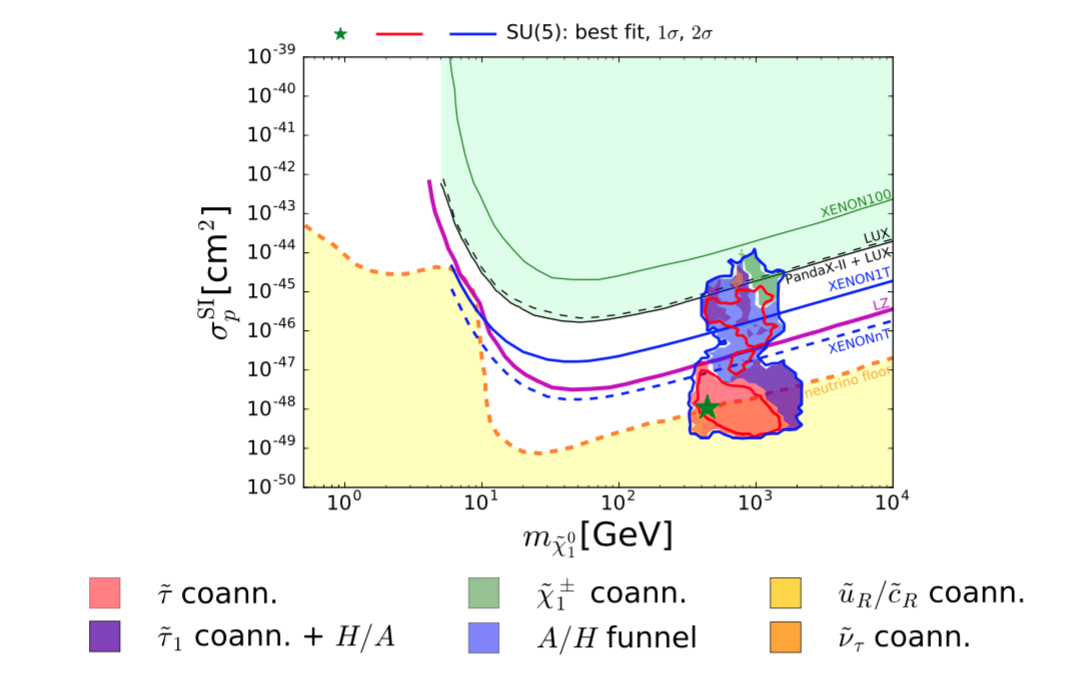
\includegraphics[width=0.9\textwidth]{./Figures/conclusions/mastercode}
  \caption{
The ($m_{\chiz}$, $\sigma_p^{\text{SI}}$) plane in the SUSY SU(5) GUT model~\cite{mastercode}.
The solid green line is the 95\% CL upper limit from the XENON100 experiment, 
and the dashed black solid line is the 95\% CL upper limit from the LUX experiment. 
The solid black line shows the 95\% CL exclusion contour for the combination 
of the PandaX-II and LUX experiments, the solid purple line shows the projected 95\% 
exclusion sensitivity of the LUX-Zeplin (LZ) experiment, the solid and dashed blue 
lines show the projected 95\% sensitivities of the XENON1T and XENONnT experiments,
respectively, and the dashed orange line shows the astrophysical neutrino 'floor`, 
below which astrophysical neutrino backgrounds dominate (yellow region). 
The determination of the 68\% and 95\% CL regions is detailed fully in Reference~\cite{mastercode}
and the colours and shadings within the 68\% and 95\% CL regions represent the dominant
DM mechanisms.}
  \label{fig:mastercode}
\end{figure}
